\documentclass[10pt,a4paper]{article}
\usepackage{hyperref}
\usepackage{graphicx}
\usepackage{setspace}
\usepackage{fontspec}
\usepackage[figurename=Fig.]{caption}
\usepackage{float}
\usepackage{polyglossia}
\setmainlanguage{english}
\setotherlanguage{arabic}
\newfontfamily\arabicfont[Script=Arabic,Scale=1.1]{Scheherazade}
\hypersetup{
    colorlinks=true,
    linkcolor=blue,
    filecolor=magenta,      
    urlcolor=blue,
}
\graphicspath{ {images/} }
\renewcommand{\figurename}{\textarabic{عکس}}
\renewcommand{\thefigure}{\arabic{figure}}
\begin{document}

\title{\textarabic{تمرین دوم یادگیری ماشین}}
\author{\textarabic{دایوش حسن پور}}
\date{}
\maketitle
\null
\vfill
\begin{center}
\textarabic{پاییز ۱۳۹۳}
\end{center}
\newpage

\begin{Arabic}
\section{\textarabic{مقدمه}}
این تمرین در مورد پیاده سازی الگوریتم های 
\end{Arabic}
\textenglish{$Q(\lambda)$\footnote{http://webdocs.cs.ualberta.ca/~sutton/book/ebook/node78.html}}
\textarabic{و}
\textenglish{$SARSA(\lambda)$\footnote{http://webdocs.cs.ualberta.ca/~sutton/book/ebook/node77.html}}
\begin{Arabic}
ولی به علت عدم توجه بنده به عبارت 
$\lambda$
در هنگام خواندن تعریف تمرین در ابتدا بنده الگوریتم های 
\end{Arabic}
\textenglish{$Q(s, a)$\footnote{http://artint.info/html/ArtInt\char`_265.html}}
\textarabic{و}
\textenglish{$SARSA(s, a)$\footnote{http://artint.info/html/ArtInt\char`_268.html}}
\begin{Arabic}
علاوه بر الگوریتم های
\textenglish{$Q(\lambda)$} و \textenglish{$SARSA(\lambda)$}
را نیز پیاده سازی کرده ام.
\section{\textarabic{معرفی برنامه}}
برنامه به زبان
\textenglish{C\#}
تحت قالب کاری
\textenglish{.Net 4.0}
تحت محیط
\textenglish{Visual Studio 2010}
نوشته شده است.
  برنامه دارای ظاهری بسیار پویا دارد که قابلیت تغییر محیط و جابجایی موقعیت های عامل و هدف و همچنین پارامتر 
  های یادگیری را به صورت گرافیکی دارا میباشد.
\begin{figure}[H]
    \centering
    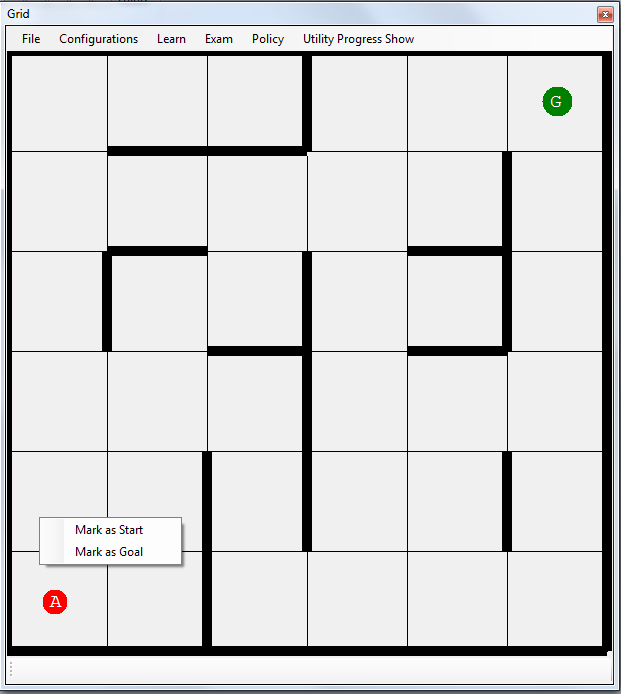
\includegraphics[width=0.5\textwidth]{init}
    \begin{center}\textarabic{
    عکس ۱: یک نمایشی از محیط برنامه که با انتخاب رو خطوط میتوان آنها را به بلوک تبدیل کرد و برعکس؛ و همچنین با راست کلیک کردن بروی خانه ها امکان انتخاب موقعیت های عامل و هدف را وجود دارد.}
    \end{center}
\end{figure}
    \subsection{\textarabic{معرفی منوهای برنامه}}
    در این قسمت به معرفی منوهای برنامه میپردازم.
        \subsubsection{File}
در منوی فایل امکان ایجاد و ذخیره کردن و بازنشانی ساختار خام محیط گذاشته شده است.
\begin{figure}[H]
    \centering
    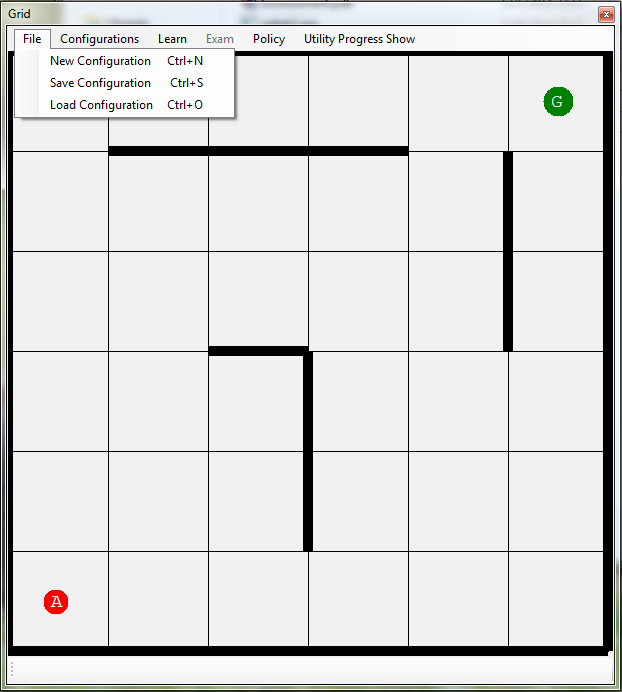
\includegraphics[width=0.5\textwidth]{file-menu}
    \begin{center}
    \textarabic{عکس ۲: منوی فایل}
    \end{center}
\end{figure}
    \subsubsection{Configurations}
    با انتخاب این منو به تنظیمات برنامه که مربوط به پارامتر های یادگیری و محیط مربوط میشود میرویم.
\begin{figure}[H]
    \centering
    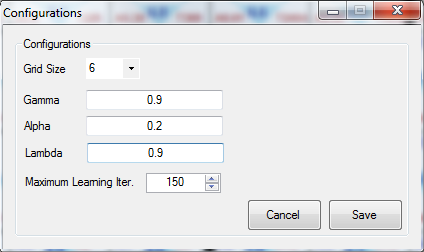
\includegraphics[width=0.5\textwidth]{conf}
    \begin{center}
    \textarabic{عکس ۳: منوی تنظیمات برنامه؛ توجه شود که اندازه شبکه همیشه مربعی در نظر گرفته شده است.}
    \end{center}
\end{figure}
    \subsubsection{Learn}
  در این منو میتوانیم یکی از ۴ الگوریتم نوشته شده را برای شبکه طراحی شده آموزش داد و نتایج بطور گرافیکی نمایش خواهد یافت که در قسمت های بعدی در مورد چگونگی تفسیر این نتایج بحث خواهد شد.
\begin{figure}[H]
    \centering
    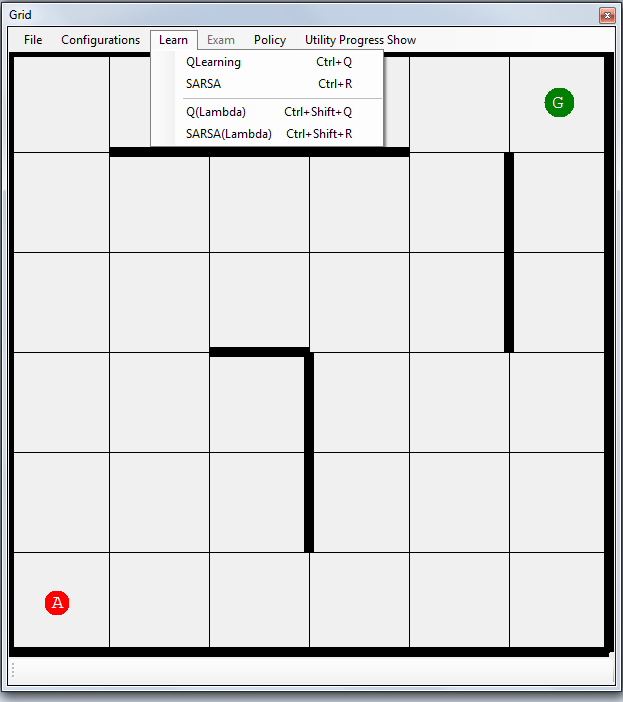
\includegraphics[width=0.5\textwidth]{learn-menu}
    \begin{center}
    \textarabic{عکس ۴: با انتخاب یکی از چهار الگوریتم؛ الگوریتم انتخاب شده شروع به یادگیری شبکه خواهد کرد.}
    \end{center}
\end{figure}
    \subsubsection{Policy}
    این منو برای ذخیره سازی و بازنشانی سیاست یادگرفته شده و سایر اطلاعاتی که پس از یادگیری شبکه بدست میاید از قیبل مقادیر سودمندی موقعیت ها و دیگر اطلاعات مرتبط مورد استفاده است که برای راحتی کار در منویی جدا قرار داده شده اند.
\begin{figure}[H]
    \centering
    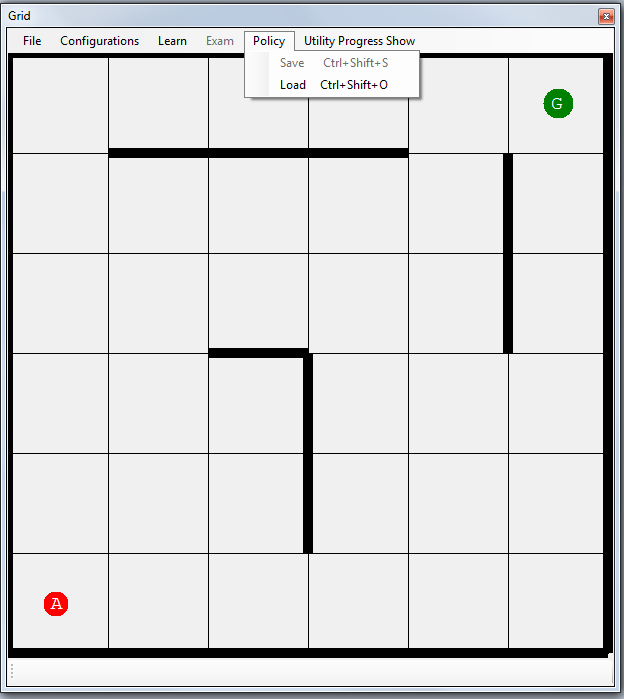
\includegraphics[width=0.5\textwidth]{policy-menu}
    \begin{center}
    \textarabic{عکس ۵: بعد از یادگیری سیاسیت و میزان سودمندی موقعیت ها میتوان آنها را ذخیره و در دفعات بعد بازنشانی کرد.}
    \end{center}
\end{figure}
    \subsubsection{Utilities Progress Show}
    برنامه در هنگام یادگیری میزان سودمندی موقعیت ها تاریخچه ای از نحوه تغییر مقادیر سودمندی تمامی موقعیت ها ذخیره میکند. که توسط این منو میتوان نحوه ی رشد یا عدم رشد سودمندی هر یک از خانه ها را به صورت جدا یا باهم(برای مقایسه) مشاهده کرد.
\begin{figure}[H]
    \centering
    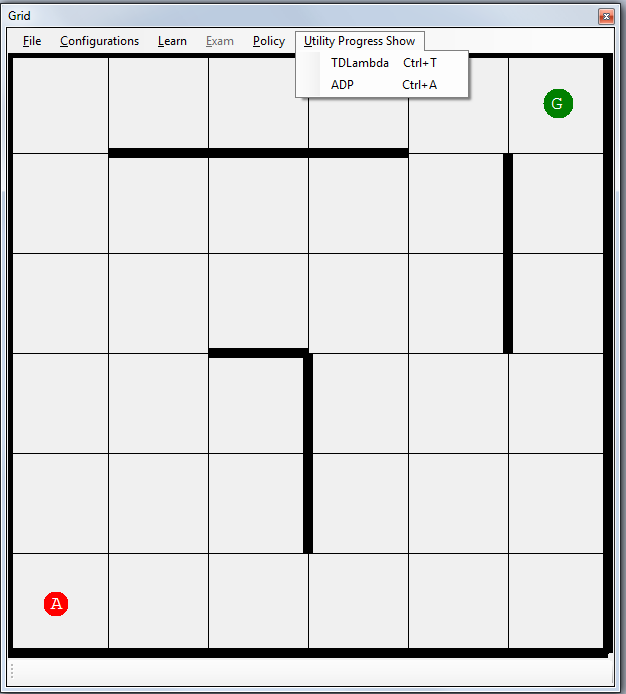
\includegraphics[width=0.5\textwidth]{util-menu}
    \begin{center}
    \textarabic{عکس ۶: با انتخاب هر یک از الگوریتم های یادگیرنده ی میزان سودمندی خانه ها میتوانیم شاهد مشاهده ی نحوه ی تغییر سودمندی موقعیت باشیم.}
    \end{center}
\end{figure}\begin{figure}[H]
    \centering
    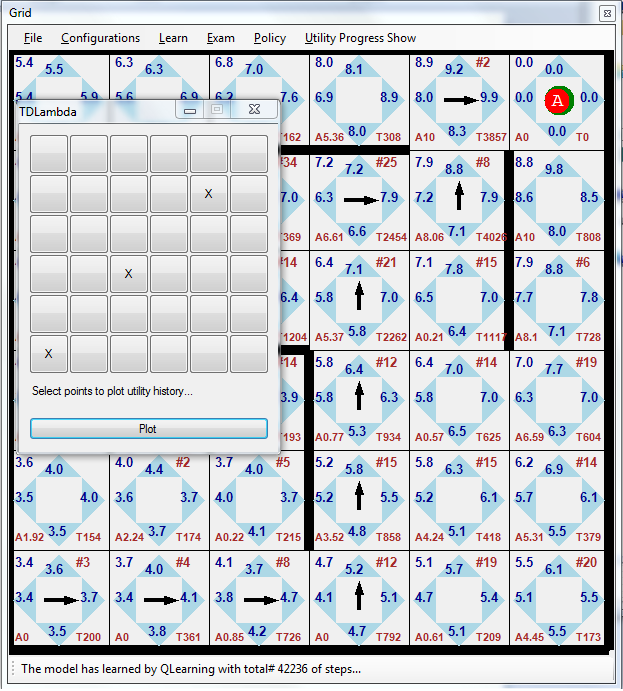
\includegraphics[width=0.5\textwidth]{util-form}
    \begin{center}
    \textarabic{عکس ۷: با انتخاب خانه های مد نظر(با هم یا به بطور تکی) می توانیم به مقایسه نحوه ی تغییر میزان سودمندی خانه ها بپردازیم.}
    \end{center}
\end{figure}
\end{Arabic}




\end{document}
